% Options for packages loaded elsewhere
\PassOptionsToPackage{unicode}{hyperref}
\PassOptionsToPackage{hyphens}{url}
%
\documentclass[
]{article}
\usepackage{amsmath,amssymb}
\usepackage{iftex}
\ifPDFTeX
  \usepackage[T1]{fontenc}
  \usepackage[utf8]{inputenc}
  \usepackage{textcomp} % provide euro and other symbols
\else % if luatex or xetex
  \usepackage{unicode-math} % this also loads fontspec
  \defaultfontfeatures{Scale=MatchLowercase}
  \defaultfontfeatures[\rmfamily]{Ligatures=TeX,Scale=1}
\fi
\usepackage{lmodern}
\ifPDFTeX\else
  % xetex/luatex font selection
\fi
% Use upquote if available, for straight quotes in verbatim environments
\IfFileExists{upquote.sty}{\usepackage{upquote}}{}
\IfFileExists{microtype.sty}{% use microtype if available
  \usepackage[]{microtype}
  \UseMicrotypeSet[protrusion]{basicmath} % disable protrusion for tt fonts
}{}
\makeatletter
\@ifundefined{KOMAClassName}{% if non-KOMA class
  \IfFileExists{parskip.sty}{%
    \usepackage{parskip}
  }{% else
    \setlength{\parindent}{0pt}
    \setlength{\parskip}{6pt plus 2pt minus 1pt}}
}{% if KOMA class
  \KOMAoptions{parskip=half}}
\makeatother
\usepackage{xcolor}
\usepackage[margin=1in]{geometry}
\usepackage{color}
\usepackage{fancyvrb}
\newcommand{\VerbBar}{|}
\newcommand{\VERB}{\Verb[commandchars=\\\{\}]}
\DefineVerbatimEnvironment{Highlighting}{Verbatim}{commandchars=\\\{\}}
% Add ',fontsize=\small' for more characters per line
\usepackage{framed}
\definecolor{shadecolor}{RGB}{248,248,248}
\newenvironment{Shaded}{\begin{snugshade}}{\end{snugshade}}
\newcommand{\AlertTok}[1]{\textcolor[rgb]{0.94,0.16,0.16}{#1}}
\newcommand{\AnnotationTok}[1]{\textcolor[rgb]{0.56,0.35,0.01}{\textbf{\textit{#1}}}}
\newcommand{\AttributeTok}[1]{\textcolor[rgb]{0.13,0.29,0.53}{#1}}
\newcommand{\BaseNTok}[1]{\textcolor[rgb]{0.00,0.00,0.81}{#1}}
\newcommand{\BuiltInTok}[1]{#1}
\newcommand{\CharTok}[1]{\textcolor[rgb]{0.31,0.60,0.02}{#1}}
\newcommand{\CommentTok}[1]{\textcolor[rgb]{0.56,0.35,0.01}{\textit{#1}}}
\newcommand{\CommentVarTok}[1]{\textcolor[rgb]{0.56,0.35,0.01}{\textbf{\textit{#1}}}}
\newcommand{\ConstantTok}[1]{\textcolor[rgb]{0.56,0.35,0.01}{#1}}
\newcommand{\ControlFlowTok}[1]{\textcolor[rgb]{0.13,0.29,0.53}{\textbf{#1}}}
\newcommand{\DataTypeTok}[1]{\textcolor[rgb]{0.13,0.29,0.53}{#1}}
\newcommand{\DecValTok}[1]{\textcolor[rgb]{0.00,0.00,0.81}{#1}}
\newcommand{\DocumentationTok}[1]{\textcolor[rgb]{0.56,0.35,0.01}{\textbf{\textit{#1}}}}
\newcommand{\ErrorTok}[1]{\textcolor[rgb]{0.64,0.00,0.00}{\textbf{#1}}}
\newcommand{\ExtensionTok}[1]{#1}
\newcommand{\FloatTok}[1]{\textcolor[rgb]{0.00,0.00,0.81}{#1}}
\newcommand{\FunctionTok}[1]{\textcolor[rgb]{0.13,0.29,0.53}{\textbf{#1}}}
\newcommand{\ImportTok}[1]{#1}
\newcommand{\InformationTok}[1]{\textcolor[rgb]{0.56,0.35,0.01}{\textbf{\textit{#1}}}}
\newcommand{\KeywordTok}[1]{\textcolor[rgb]{0.13,0.29,0.53}{\textbf{#1}}}
\newcommand{\NormalTok}[1]{#1}
\newcommand{\OperatorTok}[1]{\textcolor[rgb]{0.81,0.36,0.00}{\textbf{#1}}}
\newcommand{\OtherTok}[1]{\textcolor[rgb]{0.56,0.35,0.01}{#1}}
\newcommand{\PreprocessorTok}[1]{\textcolor[rgb]{0.56,0.35,0.01}{\textit{#1}}}
\newcommand{\RegionMarkerTok}[1]{#1}
\newcommand{\SpecialCharTok}[1]{\textcolor[rgb]{0.81,0.36,0.00}{\textbf{#1}}}
\newcommand{\SpecialStringTok}[1]{\textcolor[rgb]{0.31,0.60,0.02}{#1}}
\newcommand{\StringTok}[1]{\textcolor[rgb]{0.31,0.60,0.02}{#1}}
\newcommand{\VariableTok}[1]{\textcolor[rgb]{0.00,0.00,0.00}{#1}}
\newcommand{\VerbatimStringTok}[1]{\textcolor[rgb]{0.31,0.60,0.02}{#1}}
\newcommand{\WarningTok}[1]{\textcolor[rgb]{0.56,0.35,0.01}{\textbf{\textit{#1}}}}
\usepackage{graphicx}
\makeatletter
\def\maxwidth{\ifdim\Gin@nat@width>\linewidth\linewidth\else\Gin@nat@width\fi}
\def\maxheight{\ifdim\Gin@nat@height>\textheight\textheight\else\Gin@nat@height\fi}
\makeatother
% Scale images if necessary, so that they will not overflow the page
% margins by default, and it is still possible to overwrite the defaults
% using explicit options in \includegraphics[width, height, ...]{}
\setkeys{Gin}{width=\maxwidth,height=\maxheight,keepaspectratio}
% Set default figure placement to htbp
\makeatletter
\def\fps@figure{htbp}
\makeatother
\setlength{\emergencystretch}{3em} % prevent overfull lines
\providecommand{\tightlist}{%
  \setlength{\itemsep}{0pt}\setlength{\parskip}{0pt}}
\setcounter{secnumdepth}{-\maxdimen} % remove section numbering
\ifLuaTeX
  \usepackage{selnolig}  % disable illegal ligatures
\fi
\usepackage{bookmark}
\IfFileExists{xurl.sty}{\usepackage{xurl}}{} % add URL line breaks if available
\urlstyle{same}
\hypersetup{
  pdftitle={Adeline-Makokha\_191199-Assignment-8.R},
  pdfauthor={PC},
  hidelinks,
  pdfcreator={LaTeX via pandoc}}

\title{Adeline-Makokha\_191199-Assignment-8.R}
\author{PC}
\date{2025-05-08}

\begin{document}
\maketitle

\begin{Shaded}
\begin{Highlighting}[]
\CommentTok{\# Hospital Department Efficiency Analysis using DEA in R}

\CommentTok{\# Install Benchmarking package if not already installed}
\CommentTok{\# install.packages("Benchmarking")}
\FunctionTok{library}\NormalTok{(Benchmarking)}
\end{Highlighting}
\end{Shaded}

\begin{verbatim}
## Warning: package 'Benchmarking' was built under R version 4.4.3
\end{verbatim}

\begin{verbatim}
## Loading required package: lpSolveAPI
\end{verbatim}

\begin{verbatim}
## Warning: package 'lpSolveAPI' was built under R version 4.4.3
\end{verbatim}

\begin{verbatim}
## Loading required package: ucminf
\end{verbatim}

\begin{verbatim}
## Loading required package: quadprog
\end{verbatim}

\begin{Shaded}
\begin{Highlighting}[]
\CommentTok{\# Read hospital data}
\CommentTok{\#hospital\_data \textless{}{-} read.csv("hospital\_data.csv")}
\NormalTok{hospital\_data }\OtherTok{\textless{}{-}} \FunctionTok{read.csv}\NormalTok{(}\StringTok{"C:/Users/PC/Downloads/ADEH{-}MSC/Module 3/Module{-}3/DSA 8302 Computational Techniques in DS/week 8/hospital\_data.csv"}\NormalTok{)}


\CommentTok{\# Print raw data}
\FunctionTok{print}\NormalTok{(}\StringTok{"Hospital Department Data:"}\NormalTok{)}
\end{Highlighting}
\end{Shaded}

\begin{verbatim}
## [1] "Hospital Department Data:"
\end{verbatim}

\begin{Shaded}
\begin{Highlighting}[]
\FunctionTok{print}\NormalTok{(hospital\_data)}
\end{Highlighting}
\end{Shaded}

\begin{verbatim}
##      DMU Doctors Nurses Beds Patients SurvivalRate
## 1 Dept A      40     80  150     2000         0.97
## 2 Dept B      35     70  140     1900         0.96
## 3 Dept C      45     85  160     2100         0.98
## 4 Dept D      38     75  145     1950         0.95
\end{verbatim}

\begin{Shaded}
\begin{Highlighting}[]
\CommentTok{\# Prepare input and output matrices}
\NormalTok{inputs }\OtherTok{\textless{}{-}} \FunctionTok{as.matrix}\NormalTok{(hospital\_data[, }\FunctionTok{c}\NormalTok{(}\StringTok{"Doctors"}\NormalTok{, }\StringTok{"Nurses"}\NormalTok{, }\StringTok{"Beds"}\NormalTok{)])}
\NormalTok{outputs }\OtherTok{\textless{}{-}} \FunctionTok{as.matrix}\NormalTok{(hospital\_data[, }\FunctionTok{c}\NormalTok{(}\StringTok{"Patients"}\NormalTok{, }\StringTok{"SurvivalRate"}\NormalTok{)])}

\CommentTok{\# DEA using CCR model (constant returns to scale), input{-}oriented}
\NormalTok{dea\_ccr }\OtherTok{\textless{}{-}} \FunctionTok{dea}\NormalTok{(}\AttributeTok{X =}\NormalTok{ inputs, }\AttributeTok{Y =}\NormalTok{ outputs, }\AttributeTok{RTS =} \StringTok{"crs"}\NormalTok{, }\AttributeTok{ORIENTATION =} \StringTok{"in"}\NormalTok{)}
\NormalTok{hospital\_data}\SpecialCharTok{$}\NormalTok{CCR\_Efficiency }\OtherTok{\textless{}{-}}\NormalTok{ dea\_ccr}\SpecialCharTok{$}\NormalTok{eff}

\CommentTok{\# DEA using BCC model (variable returns to scale), input{-}oriented}
\NormalTok{dea\_bcc }\OtherTok{\textless{}{-}} \FunctionTok{dea}\NormalTok{(}\AttributeTok{X =}\NormalTok{ inputs, }\AttributeTok{Y =}\NormalTok{ outputs, }\AttributeTok{RTS =} \StringTok{"vrs"}\NormalTok{, }\AttributeTok{ORIENTATION =} \StringTok{"in"}\NormalTok{)}
\NormalTok{hospital\_data}\SpecialCharTok{$}\NormalTok{BCC\_Efficiency }\OtherTok{\textless{}{-}}\NormalTok{ dea\_bcc}\SpecialCharTok{$}\NormalTok{eff}

\CommentTok{\# Print efficiency results}
\FunctionTok{print}\NormalTok{(}\StringTok{"DEA Efficiency Scores (CCR and BCC):"}\NormalTok{)}
\end{Highlighting}
\end{Shaded}

\begin{verbatim}
## [1] "DEA Efficiency Scores (CCR and BCC):"
\end{verbatim}

\begin{Shaded}
\begin{Highlighting}[]
\FunctionTok{print}\NormalTok{(hospital\_data[, }\FunctionTok{c}\NormalTok{(}\StringTok{"DMU"}\NormalTok{, }\StringTok{"CCR\_Efficiency"}\NormalTok{, }\StringTok{"BCC\_Efficiency"}\NormalTok{)])}
\end{Highlighting}
\end{Shaded}

\begin{verbatim}
##      DMU CCR_Efficiency BCC_Efficiency
## 1 Dept A      0.9824561              1
## 2 Dept B      1.0000000              1
## 3 Dept C      0.9671053              1
## 4 Dept D      0.9909256              1
\end{verbatim}

\begin{Shaded}
\begin{Highlighting}[]
\CommentTok{\# Plot CCR Efficiency}
\FunctionTok{barplot}\NormalTok{(hospital\_data}\SpecialCharTok{$}\NormalTok{CCR\_Efficiency, }\AttributeTok{names.arg=}\NormalTok{hospital\_data}\SpecialCharTok{$}\NormalTok{DMU,}
        \AttributeTok{col=}\StringTok{"steelblue"}\NormalTok{, }\AttributeTok{ylim=}\FunctionTok{c}\NormalTok{(}\DecValTok{0}\NormalTok{,}\FloatTok{1.1}\NormalTok{), }\AttributeTok{main=}\StringTok{"CCR Efficiency Scores"}\NormalTok{,}
        \AttributeTok{ylab=}\StringTok{"Efficiency Score"}\NormalTok{, }\AttributeTok{las=}\DecValTok{2}\NormalTok{)}
\end{Highlighting}
\end{Shaded}

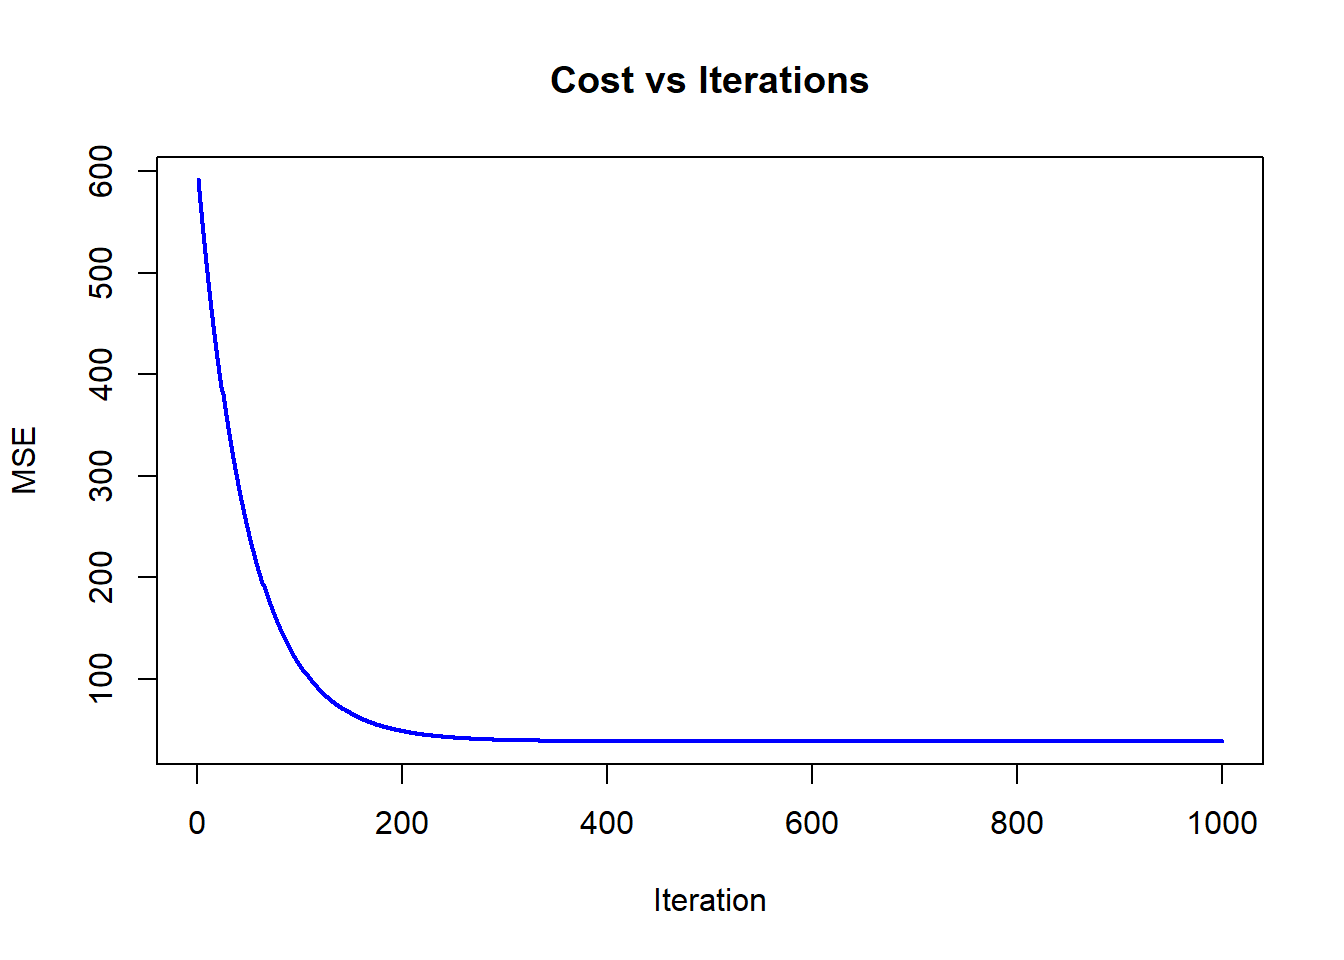
\includegraphics{Adeline-Makokha_191199-Assignment-8_files/figure-latex/unnamed-chunk-1-1.pdf}

\begin{Shaded}
\begin{Highlighting}[]
\CommentTok{\# Plot BCC Efficiency}
\FunctionTok{barplot}\NormalTok{(hospital\_data}\SpecialCharTok{$}\NormalTok{BCC\_Efficiency, }\AttributeTok{names.arg=}\NormalTok{hospital\_data}\SpecialCharTok{$}\NormalTok{DMU,}
        \AttributeTok{col=}\StringTok{"darkgreen"}\NormalTok{, }\AttributeTok{ylim=}\FunctionTok{c}\NormalTok{(}\DecValTok{0}\NormalTok{,}\FloatTok{1.1}\NormalTok{), }\AttributeTok{main=}\StringTok{"BCC Efficiency Scores"}\NormalTok{,}
        \AttributeTok{ylab=}\StringTok{"Efficiency Score"}\NormalTok{, }\AttributeTok{las=}\DecValTok{2}\NormalTok{)}
\end{Highlighting}
\end{Shaded}

\includegraphics{Adeline-Makokha_191199-Assignment-8_files/figure-latex/unnamed-chunk-1-2.pdf}

\end{document}
